\section{Data Models}\label{sec:dataModels}
Given the Tycho-2 catalog of stars, how can we model our data our data for efficient spatial queries on a static
database?

\subsection{Relational Data Model}\label{subsec:relationalDataModel}
The relational data model is the most popular data abstraction, and arguably the most natural.
Here data is stored in $n$-dimensional vectors known as tuples.
The schema is defined before data is added, meaning that each tuple of a given set has the same length.
If thought of as a table, the number of columns is fixed while the number of rows is variable.
Interaction between this model involves the use of relational algebra (typically implemented as SQL).

In terms of distributed relational DBMSs, most implementations are consistent, available, but not partition tolerant.
This means that every read will always receive the most recent write.
Given that our database is static, the biggest concern is partition tolerance.
Our system may not operate with message loss across a cluster of computers (nodes).

\subsection{Column Family Data Model}\label{subsec:columnFamilyDataModel}
\begin{figure}
    \centering{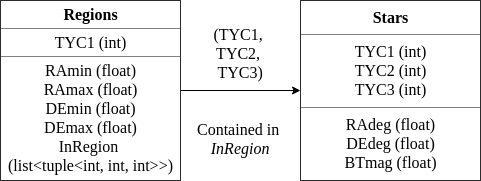
\includegraphics[scale=0.5]{images/cassandra-data-model.png}}
    \caption{Depiction of data model used with Cassandra.
    There exists a \textit{Stars} column family indexed by \texttt{TYC1, TYC2, TYC3}, and a \textit{Regions} column
    family indexed by \texttt{TYC1}.
    Stars exist in regions if they share the same \texttt{TYC1} number.}
    \label{fig:cassandraDataModel}
\end{figure}

The column family data model can be very loosely thought of as the segmentation of a relational table into several two
column tables consisting of a single attribute of the original table and a primary key based off this attribute.
These segmented tables can then be grouped into a column family, which represents a group of columns indexed by the
same primary key.
This segmentation is useful for allowing denormalization, meaning that the schema does not have to be defined before
data insertion and that each primary key does not have to map the same amount of columns as other keys.
Column family models are known for this denormalization and efficient querying, accessing only the columns required for
the query itself.
Cons here include restrictive queries, as columns can only be accessed using their primary key.

\textit{Apache Cassandra} is the column store database that is being tested here, and is a form of a
\textit{distributed} DBMS\@.
Cassandra itself is available and partition tolerant, but not consistent.
Data in a Cassandra cluster is hash partitioned by the primary key with the additional option of being replicated
across the cluster.
Cassandra's querying language CQL allows for queries without the primary key, but at the cost of performance.

The data model being implemented with Cassandra involves two column families: \textit{Regions} and \textit{Stars}.
The \textit{Stars} family has six columns:
\begin{multicols}{3}
    \noindent
    \begin{itemize}
        \item[] \texttt{TYC1}
        \item[] \texttt{TYC2}
        \item[] \texttt{TYC3}
        \item[] \texttt{RAmdeg}
        \item[] \texttt{DEmdeg}
        \item[] \texttt{BTmag}
    \end{itemize}
\end{multicols}
where \texttt{TYC1, TYC2, TYC3} represent the star's ID, \texttt{RAmdeg, DEmdeg} represent the star's position, and
\texttt{BTmag} represents the magnitude of the star.
This is depicted in~\autoref{fig:cassandraDataModel}.
The primary key for this family is the GSC region \texttt{TYC1}, with \texttt{TYC2, TYC3} as secondary clustering
keys.
Efficient queries for stars should involve the primary key \texttt{TYC1}.

The \textit{Regions} family has five columns:
\begin{multicols}{3}
    \noindent
    \begin{itemize}
        \item[] \texttt{TYC1}
        \item[] \texttt{RAmin}
        \item[] \texttt{RAmax}
        \item[] \texttt{DEmin}
        \item[] \texttt{DEmax}
    \end{itemize}
\end{multicols}
where \texttt{TYC1} represents the region ID, (\texttt{RAmin, RAmax}) represent the right ascension limits, and
(\texttt{DEmin, DEmax}) represent the declination limits.
Star exist in the same region if they share the same \texttt{TYC1} region ID\@, which is also the primary key for
the \textit{Region} family.
Efficient region queries will use only the \texttt{TYC1} primary key.

%To query for all attributes of stars within a region, we first query for the \texttt{InRegion} column in the
%\textit{Region} family given the \texttt{TYC1}.
%Every star returned from this query is then used to search all columns of the \textit{Stars} family.

\subsection{Graph Data Model}\label{subsec:graphDataModel}
\begin{figure}
    \centering{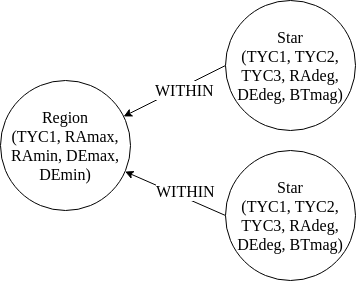
\includegraphics[scale=0.5]{images/neo4j-data-model.png}}
    \caption{Depiction of data model used with Neo4J.
    There exists a collection of \textit{Star} nodes and \textit{Region} nodes, each of which are related by the
    \texttt{WITHIN} relationship.}
\end{figure}

Relative to the relational data model, the graph data model focuses on the relationship between various tuples.
Here data is stored in nodes as attributes, and relationships are stored as edges between nodes.
Data is accessed by searching for nodes or edges, and traversing the graph.
Compared to the relational data model, graph data models shine in relationship querying and denormalization.
Compared to the column family where data can easily be partitioned across nodes, a graph data model does not allow
for the same amount of parallelism.

\textit{Neo4J} is the graph database that is being tested here, and is also a form of a distributed DBMS\@.
The Neo4J setup that was tested here is available and consistent, but not partition tolerant (like a typical
distributed RDBMS).
Because data in a Neo4J graph cannot be partitioned like Cassandra, every node in a cluster is a full replica.

The data model being implemented here involves two types of nodes: \textit{Region} and \textit{Star} nodes.
A \textit{Star} node has the same attributes as the columns in the Cassandra \textit{Stars} family.
\textit{Regions} have all attributes in the columns of the \textit{Regions} family.
A \texttt{WITHIN} relationship is established between all \textit{Star} nodes that exist in a region.

%To query for all attributes for a star within a region, we first search for the \textit{Region} node that matches
%some \texttt{TYC1} ID\@.
%The next step involves traversing all \texttt{WITHIN} edges to each \textit{Star} node and returning the attributes.